\chapter{Background}
\label{Chapt2}
\section{draft Paragraphs}
1. Domain Name System Security and Privacy: A Contemporary Survey

The Domain Name System (DNS) plays a role, in the functioning of the Internet as it helps translate user domain names into IP addresses. However this system has faced security and privacy challenges over time. The article titled "Domain Name System Security and Privacy; A Contemporary Survey" on ScienceDirect provides an examination of these issues. It emphasizes the importance of DNS in ensuring Internet operations while also highlighting the vulnerabilities that malicious individuals can exploit. Moreover the article explores solutions and approaches that have been suggested to enhance DNS security and privacy. With the Internet constantly evolving, safeguarding the reliability and integrity of DNS becomes increasingly vital.\cite{sciencedirect2023dns}  This survey serves as a resource, for researchers and professionals seeking to comprehend and tackle concerns related to DNS security and privacy.


2. DNS Abuse Institute

The DNS Abuse Institute is an organization that focuses on combating DNS abuse and ensuring the safety and security of the Domain Name System. Their main goal is to assist the internet community in identifying, reporting and mitigating instances of DNS abuse. They place emphasis on establishing practices supporting DNS related research and facilitating data sharing. \cite{dnsabuseinstitute2023} The institute takes an approach by introducing solutions like "Compass Dashboards," which provide essential data to registries and registrars. Additionally they regularly publish reports and bulletins such, as the "DNSAI 2022 Annual Report" and the "DNSAI Bulletin 2023 04; Account Take Overs " offering insights, into the state of DNS abuse and the steps being taken to combat it.


3. DNS Privacy in Practice and Preparation


The Domain Name System (DNS) plays a role, in the Internet by helping to convert domain names into IP addresses. As online privacy becomes more important there have been improvements made to the DNS to ensure private communication. A paper called "DNS Privacy in Practice and Preparation " published in the proceedings of the International Conference on Emerging Networking Experiments And Technologies explores these advancements. It specifically focuses on how Transport Layer Security (TLS) and Hypertext Transfer Protocol Secure (HTTPS)'re implemented for DNS queries. The research provides insights into how DNS over TLS (DoT) and DNS over HTTPS (DoH)'re being used by open resolvers and authoritative DNS servers. The paper points out that while adoption of DoT and DoH is limited major public DNS service providers have already integrated them. \cite{acm2023dnsprivacy} Additionally the research emphasizes the importance of TCP Fast Open (TFO) in reducing latency for TCP based DNS queries highlighting the need, for adoption to ensure performance when using enhanced DNS privacy measures.


4. SEPTEMBER 2022 REPORT - DNS Abuse Institute

The DNS Abuse Institutes "September 2022 Report" presents an overview of the status of DNS abuse. This report showcases the institutes dedication to identifying, reporting and mitigating instances of DNS abuse. Although direct access, to the reports content is not available it likely delves into cases of DNS abuse observed in September 2022 the actions taken to address them and recommendations for implementing practices. Reports like these are incredibly valuable for individuals involved in the domain name industry as they provide insights into emerging threats and how effectively current mitigation strategies are working.\cite{dnsai2022report} The periodic reports from the DNS Abuse Institute serve as a reference point, for understanding the evolving landscape of DNS abuse and the collective efforts being made to combat it.


5. ICANN Reports DNS Abuse is Trending Downward Globally

The press release issued by ICANN titled "ICANNs Report Reveals Decreasing Global Trend of DNS Abuse" delivers encouraging news regarding the state of DNS abuse. Over the course of the four years there has been a decrease, in instances of global DNS abuse showcasing the effectiveness of measures implemented by stakeholders within the domain name industry.\cite{icann2022dnsabuse} It is highly likely that ICANNs report provides in depth analysis, on this decline offering data and insights regarding the impacted regions the types of abuse that have experienced significant reductions and the strategies that have proven particularly successful in combating DNS abuse.


6. Summary of DNS Over HTTPS Abuse

The article titled "A Summary of DNS Over HTTPS Abuse”, from IEEE Xplore explores the use of the DNS over HTTPS (DoH) protocol. While DoH aims to address privacy concerns regarding DNS queries it is not without security risks. The article likely discusses the benefits of DoH in safeguarding user privacy through DNS queries. However it also emphasizes the security threats that come with its adoption. These threats may involve misuse by individuals, difficulties in monitoring DNS traffic, for domains and potential vulnerabilities within the protocol itself.\cite{ieee2023dohabuse} Overall this paper offers an overview of how DoH balances privacy improvements and security challenges.


7. A Survey on DNS Encryption: Current Development, Malware Misuse, and Inference Techniques

The research paper titled "An In Depth Look, at DNS Encryption; Progress, Exploitation by Malware and Methods for Detection" published on arXiv provides an overview of the domain name system (DNS) and its importance in the functioning of the Internet. The paper highlights the risks posed by individuals particularly in relation to DNS encryption. It likely discusses advancements made in DNS encryption techniques how malware exploits these techniques and various methods that can be used to identify and address threats. \cite{arxiv2023dnsencryption} This survey is a resource, for researchers, professionals and policymakers seeking to understand the evolving landscape of DNS encryption and the associated security challenges.




8. Webinar: Understanding and Combating DNS Abuse - Encouraging Best Practice

The ICANN Stakeholder Assembly Webinar Series hosts a webinar called "Understanding and Combating DNS Abuse – Encouraging Best Practice." This session features Rowena Schoo and Graeme Bunton from the DNS Abuse Institute, who discuss the trends and perspectives, on DNS abuse. The DNS Abuse Institute, established in 2021 aims to provide research that's trustworthy and transparent with the ultimate goal of reducing DNS abuse and promoting best practices within the DNS community. During the webinar they highlight the scope of their work their measurement initiatives and the current state of DNS abuse with a focus on issues to the UK. \cite{icann2023webinar} Nigel Hickson, Senior Advisor, at the Department of Culture, Media and Sport (DCMS) representing the UK government to ICANNs Governmental Advisory Committee (GAC) also shares insights during this session.



\section{Different Forms of DNS Abuse}

\subsection{Phishing}
\begin{itemize}
    \item \textbf{Description:} Phishing is a technique aimed at deceiving individuals by creating website addresses that mimic those of companies, to trick users into revealing sensitive information such as login credentials, credit card numbers, or personal identification information.\cite{webinarcare2023dnsstats}
    \item \textbf{Mechanism:} This deception often occurs through emails or messaging services that direct users to websites resembling authentic ones.\cite{jakobsson2006phishing}
    \item \textbf{Impact:} Victims may suffer identity theft, financial fraud, and security compromise.
\end{itemize}

\subsection{Confusable Domains (Typosquatting)}
\begin{itemize}
    \item \textbf{Description:} Registering domain names that look visually similar to popular websites, taking advantage of typing errors or character similarities.\cite{inta2023dnstypo}
    \item \textbf{Mechanism:} Users may accidentally visit these websites when making a typo in a URL, potentially exposing them to malware or phishing attempts.
    \item \textbf{Impact:} Deception of users and potential harm to brand reputation.\cite{edelman2008typosquatting}
\end{itemize}

\subsection{Domain Hijacking}
\begin{itemize}
    \item \textbf{Description:} Unauthorized acquisition of domain names by exploiting security vulnerabilities in the domain registration system.\cite{inta2023dnstypo}
    \item \textbf{Mechanism:} Attackers may use tactics like social engineering, phishing, or exploiting security loopholes to gain control over a domain.
    \item \textbf{Impact:} Loss of website control, redirection to malicious sites, and potential data breaches.
\end{itemize}

\subsection{Botnets}
\begin{itemize}
    \item \textbf{Description:} Botnets involve controlling a group of computers infected with malware, used to carry out attacks or spread spam and malware.\cite{citpyour}
    \item \textbf{Mechanism:} Malware infects unsuspecting users’ computers, incorporating them into a network under the attacker's control.
    \item \textbf{Impact:} Can result in large-scale DDoS attacks, mass spam campaigns, and widespread malware dissemination.
\end{itemize}

\subsection{Fast Flux Hosting}
\begin{itemize}
    \item \textbf{Description:} A technique used to conceal the location of websites associated with phishing and malware distribution.\cite{lin2013genetic}
    \item \textbf{Mechanism:} Involves a network of compromised hosts that regularly modify DNS records to evade detection.
    \item \textbf{Impact:} Makes tracking and shutting down malicious sites difficult.
\end{itemize}

\subsection{Domain Generation Algorithms (DGA)}
\begin{itemize}
    \item \textbf{Description:} DGAs generate domain names that act as meeting points for botnets.\cite{antonakakis2012throw}
    \item \textbf{Mechanism:} Malicious software uses algorithms to generate a sequence of domain names for command-and-control servers.
    \item \textbf{Impact:} Adds complexity to efforts aimed at disrupting botnet command and control channels.
\end{itemize}


\section{How DNS Abuse Harms Users}

\subsection{Identity Theft}
\begin{itemize}
    \item \textbf{Phishing:} Phishing attacks often use domain names that imitate legitimate websites, fooling users into providing sensitive information such as usernames, passwords, or financial details, leading to potential identity theft.\cite{godaddy2023dnsabuse, jakobsson2006phishing}
\end{itemize}

\subsection{Financial Loss}
\begin{itemize}
    \item \textbf{Deceptive Transactions:} Users may be tricked into making payments to deceptive websites or unknowingly disclose their credit card information, resulting in financial losses.\cite{godaddy2023dnsabuse, bohme2013economics}
\end{itemize}

\subsection{Data Breach}
\begin{itemize}
    \item \textbf{Malware:} Malicious software spread through compromised DNS systems can allow unauthorized access to corporate data, leading to data breaches.\cite{icann2022dnsabusetrends, fowler2016data}
\end{itemize}

\subsection{System Compromise}
\begin{itemize}
    \item \textbf{Malware Infection:} Systems infected with malware due to DNS abuse can be exploited for further attacks, including the creation of botnets or the distribution of ransomware, resulting in system compromise.\cite{dotmagazine2022dnsabuse, saxe2018malware}
\end{itemize}

\section{Future Dangers of DNS Abuse}

\subsection{Increased Sophistication}
\begin{itemize}
    \item \textbf{Evolving Techniques:} Cyber attackers are constantly developing more sophisticated techniques to exploit DNS, such as advanced phishing schemes and malware distribution.\cite{icann2022dnsabusetrends, wrightson2014advanced}
\end{itemize}

\subsection{IoT Vulnerabilities}
\begin{itemize}
    \item \textbf{Expanding Vulnerabilities:} The widespread adoption of Internet of Things (IoT) devices, which often lack robust security measures, presents a growing target for DNS-based attacks.\cite{circleid2020dnstrends, mahmoud2015internet}
\end{itemize}

\subsection{Infrastructure Attacks}
\begin{itemize}
    \item \textbf{DNS as a Prime Target:} Attacks on DNS infrastructure can disrupt internet services on a large scale, including DDoS attacks targeting DNS providers or exploiting weaknesses in DNS protocols.\cite{dotmagazine2022dnsabuse, dooley2017dns}
\end{itemize}

\subsection{Deepfakes and AI}
\begin{itemize}
    \item \textbf{AI-Enhanced Phishing:} The use of AI technologies, such as deepfakes, has made phishing attacks more convincing and deceptive, manipulating audio and video content to impersonate trusted entities.\cite{icann2022dnsabusetrends, schick2020deep}
\end{itemize}

\subsection{Cloud Computing Vulnerabilities}
\begin{itemize}
    \item \textbf{Targeting Cloud Services:} As organizations increasingly rely on cloud-based services, cybercriminals are exploiting DNS vulnerabilities to attack these platforms, potentially leading to data breaches and service disruptions.\cite{mather2009cloud}
\end{itemize}

\subsection{Mobile Device Exploitation}
\begin{itemize}
    \item \textbf{Mobile DNS Attacks:} The rising usage of mobile devices has led cybercriminals to target smartphones and tablets through DNS-based attacks, which can lead to data theft and the spread of malware.\cite{au2016mobile}
\end{itemize}

\subsection{Cryptocurrency and Blockchain Exploitation}
\begin{itemize}
    \item \textbf{Crypto-Related DNS Attacks:} Attackers could exploit DNS vulnerabilities to redirect users to fake cryptocurrency exchanges or blockchain platforms, leading to financial fraud and theft of digital assets.\cite{bashir2019advanced}
\end{itemize}

\subsection{Political and Information Warfare}
\begin{itemize}
    \item \textbf{DNS in Cyber Warfare:} The manipulation of domain name systems can be used to spread misinformation or disrupt services during significant political events, serving as a tool for political and information warfare.\cite{chapple2021cyberwarfare}
\end{itemize}

\subsection{Exploiting Emerging Technologies}
\begin{itemize}
    \item \textbf{Abuse in New Tech Domains:} As new technologies such as 5G, AI, and quantum computing advance, tactics involving DNS abuse are likely to evolve, potentially leading to more sophisticated attacks.\cite{brunner2021cybersecurity}
\end{itemize}

\subsection{Supply Chain Attacks}
\begin{itemize}
    \item \textbf{DNS in Supply Chain Compromise:} DNS manipulation can also be employed as part of supply chain attacks, targeting software updates or cloud-based services to compromise organizations.\cite{boyson2014cyber}
\end{itemize}

\section{Mitigation of DNS Abuse}
\begin{enumerate}
    \item \textbf{Monitoring and Reporting}
    \begin{itemize}
        \item Implementation: Use automated systems to monitor the registration of domain names for patterns that may indicate DNS abuse \cite{icannndnssec}. Establish procedures for reporting activities to authorities or cybersecurity organizations \cite{lucas2021tls}.
    \end{itemize}
    \item \textbf{Security Awareness Training}
    \begin{itemize}
        \item Implementation: Develop training programs for users and IT staff with a focus on recognizing phishing attempts, practicing browsing habits, and understanding DNS security.
    \end{itemize}
    \item \textbf{DNS Security Extensions (DNSSEC)}
    \begin{itemize}
        \item Implementation: Deploy DNSSEC to ensure the integrity of DNS data. This involves signing DNS records to protect against modifications and DNS spoofing.
    \end{itemize}
    \item \textbf{Multi-Factor Authentication (MFA)}
    \begin{itemize}
        \item Implementation: Enforce Multi-Factor Authentication (MFA) for domain registrars and interfaces used for managing DNS \cite{icannndnssec}. This adds a layer of security beyond passwords, helping prevent unauthorized domain transfers or alterations \cite{moghaddam2014ecco}.
    \end{itemize}
    \item \textbf{Blacklisting and Takedown Services}
    \begin{itemize}
        \item Implementation: Collaborate with cybersecurity firms to identify and blacklist domains engaged in malicious activities. Establish response teams dedicated to taking down domains involved in DNS abuse.
    \end{itemize}
    \item \textbf{Collaboration}
    \begin{itemize}
        \item Implementation: Foster collaboration among internet service providers (ISPs), domain registrars, governments, and cybersecurity organizations. Share intelligence and best practices to collectively enhance defense against DNS abuse \cite{skopik2017collaborative}.
    \end{itemize}
    \item \textbf{Regular Audits}
    \begin{itemize}
        \item Implementation: Conduct security audits of domain registrations and DNS configurations to verify their security and ensure they have not been compromised \cite{coronado2014auditing}.
    \end{itemize}
    \item \textbf{Machine Learning}
    \begin{itemize}
        \item Implementation: Utilize AI and machine learning algorithms to analyze patterns in DNS traffic and proactively predict instances of DNS abuse \cite{icannndnssec}. This proactive approach enables the identification of threats before they materialize \cite{tsukerman2019machine}.
    \end{itemize}
    \item \textbf{Geo-Blocking and IP Filtering}
    \begin{itemize}
        \item Implementation: Deploy geo-blocking and IP filtering techniques to limit access to DNS services from regions that have a history of DNS abuse. This can reduce the risk of attackers utilizing these services to carry out malicious activities or distribute malware \cite{meeseedited}.
    \end{itemize}
    \item \textbf{Enhanced Domain Validation Procedures}
    \begin{itemize}
        \item Implementation: Enhance the domain registration process by implementing validation procedures. This may involve verifying the identity of individuals or organizations registering domains, especially for domains that resemble brands or fall into sensitive categories. By taking these measures, we can strengthen security and mitigate risks associated with fraudulent domain registrations.
    \end{itemize}
\end{enumerate}





\chapter{Figures, Tables, Referencing}

It is very important to properly refer in the text to any figures, tables or previously published work that you are discussing. Adequate and consistent referencing is one of the criteria which will be used to assess your project report.

\section{Figures}
Graphs, pictures and other images should be included in your report as a numbered, captioned figure. An example is given in Figure \ref{veldis}.

%%%%%%%%%%%%%%%%%%%%%%%%%%%%%%%%%%%%%%%%
\begin{figure}[h]
      \centering
      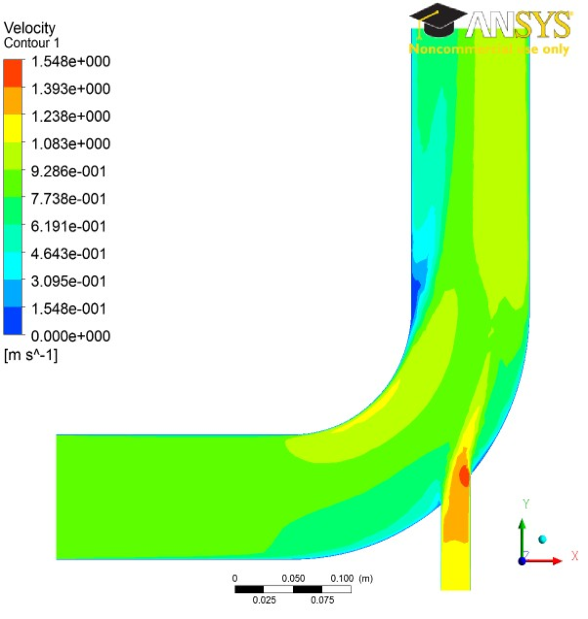
\includegraphics{background/5e1-1.pdf}
      \caption{Velocity distribution on the mid-plane for an inlet velocity for case 1.}
      \label{veldis}
\end{figure}
%%%%%%%%%%%%%%%%%%%%%%%%%%%%%%%%%%%%%%%%

The figure and caption should be centred. The figure numbering starts at 1 at the beginning of each chapter. The caption should provide a brief description of what is being shown. The figure should appear in the document after it is referred to in the text. No figure should be included which is not referred to in the text. Ensure that the size and resolution of images imported from software are sufficient to read any text.

\section{Tables}
Tables are an important way of displaying your results. Table \ref{tab:treatments} is a sample table, adapted from the Master/Doctoral Thesis template at \url{http://www.latextemplates.com/cat/theses}, which was generated with this code:

{\footnotesize
\begin{verbatim}
\begin{table}[b]
\caption{The effects of treatments X and Y on the four groups studied.}
\label{tab:treatments}
\centering
\begin{tabular}{l l l}
\toprule
\textbf{Groups} & \textbf{Treatment X} & \textbf{Treatment Y} \\\midrule
1 & 0.2 & 0.8\\
2 & 0.17 & 0.7\\
3 & 0.24 & 0.75\\
4 & 0.68 & 0.3\\
\bottomrule\\
\end{tabular}
\end{table}
\end{verbatim}
}

\begin{table}[b]
\caption{The effects of treatments X and Y on the four groups studied.}
\label{tab:treatments}
\centering
\begin{tabular}{l l l}
\toprule
\textbf{Groups} & \textbf{Treatment X} & \textbf{Treatment Y} \\
\midrule
1 & 0.2 & 0.8\\
2 & 0.17 & 0.7\\
3 & 0.24 & 0.75\\
4 & 0.68 & 0.3\\
\bottomrule\\
\end{tabular}
\end{table}

Tables are numbered in the same way as figures. Typically tables also have a short caption, but this is not universally true. The number and caption appear above the table, not below as with figures. Again, no table should appear in the report which has not been referred to in the text. Tables should come after they are discussed in the text. The exact formatting of the table depends somewhat on the content of the table, but in general, the text in the table should be the same font and size as the main text. 

\section{Equations}
All equations should be numbered sequentially. The numbering restarts automatically at the beginning of each chapter, and contains the number of the chapter alongside the equation number. Unlike figures and tables, you may not need to refer to every equation in the text. You should take care to format equations properly. Do no simply try to use plain text. Use the equation layout facilities. An example of how equations should appear is shown in \eqref{sampleequation}. Here is the code for it:

{\footnotesize
\begin{verbatim}
\begin{equation}
\textrm{div}(\underline{u}) = \frac{\delta u}{\delta x} + \frac{\delta v}{\delta y} +
        \frac{\delta w}{\delta z} = 0
\label{sampleequation}
\end{equation} 
\end{verbatim}
}

\begin{equation}
\textrm{div}(\underline{u}) = \frac{\delta u}{\delta x} + \frac{\delta v}{\delta y} + \frac{\delta w}{\delta z} = 0
\label{sampleequation}
\end{equation} 

\section{Referencing published work}
It is important to give appropriate credit to other people for the work that they have shared through publications. In fact, you must sign a declaration in your report stating that you understand the nature of plagiarism. As well as avoiding plagiarism, citing results or data from the literature can strengthen your argument, provide a favourable comparison for your results, or even demonstrate how superior your work is.

There are many styles to reference published work. For example, the parenthetical style (which is also called the \emph{Harvard style}) uses the author and date of publication (e.g. ``Smith and Jones, 2001''). There is also the Vancouver style (or the \emph{citation sequence style}). In the IEEE style, which is used in this document in the default setup, the publications are cited using bracketed numbers which refer to the list in the References section at the end of the report. The references are listed in the order that they are cited in the report. A variant is \emph{name sequence style}, in which the publications are referenced by number, but the list is arranged alphabetically. The following paragraph shows the use of the IEEE style: 

\begin{quote}
Several studies have examined the sound field around tandem cylinders generated by flow\cite{fitzpatrick2003flow,finnegan2010experimental}, while other investigations have focused on the effect of an applied sound field on the flow\cite{hall2003vortex}. Papers from conference proceedings\cite{jordan2001array}, books\cite{paidoussis2010fluid} and technical reports\cite{reyes2007power} can be dealt with in the same style.
\end{quote}

The IEEE style has the advantage that it is a little more compact in the text and does not distract from the flow of the sentence if there are a lot of citations. However, it has the disadvantage that it is not immediately clear to the reader what particular work has been referenced. You can use author names directly and discuss the work of Finnegan et al. \cite{finnegan2010experimental} similar to this sentence to make it more readable. 

It actually does not matter which particular referencing style is used as long as three important considerations are observed:
\begin{itemize}
\item the referencing style used throughout the document is consistent;
\item all material used or discussed in the text is properly cited;
\item nothing is included in the reference list that has not been cited.
\end{itemize}

Check with your supervisor as they may have a strong opinion on what you should use

This template has a suitable referencing style already set up -- you should use it and use the built-in BibTeX system to manage your references. See above for examples of how to cite a reference and look in the \texttt{sample.bib} file to see BibTeX references. It is strongly recommended that you use a bibliographic tool, such as EndNote (check out https://www.tcd.ie/library/support/endnote/), as this will facilitate compliance with these three requirements. Endnote can help you build you .bib file. Remember \href{http://scholar.google.com}{Google Scholar} and other search engines will give you BibTeX references for lots of academic publications. Be aware that Web of Science is more reliable for giving the full record for the BibTeX entry. Otherwise, you can easily make up your own based on the examples in that file.